\documentclass{article}

\usepackage{pgf}
\usepackage{tikz}
\usetikzlibrary{arrows,automata}
\usepackage[latin1]{inputenc}
\usepackage{verbatim}
\usepackage{tabularx}
\usepackage{amsmath}

\begin{document}
    \begin{center}
        \begin{huge}
            Praktikum Theoretische Informatik\\
            \vspace{5mm}
            Aufgabenblatt 2: L\"osung
        \end{huge}
    \end{center}
    \flushright{Lukas Pensler und Simon Struck}
    \flushleft
    \vspace{1cm}
    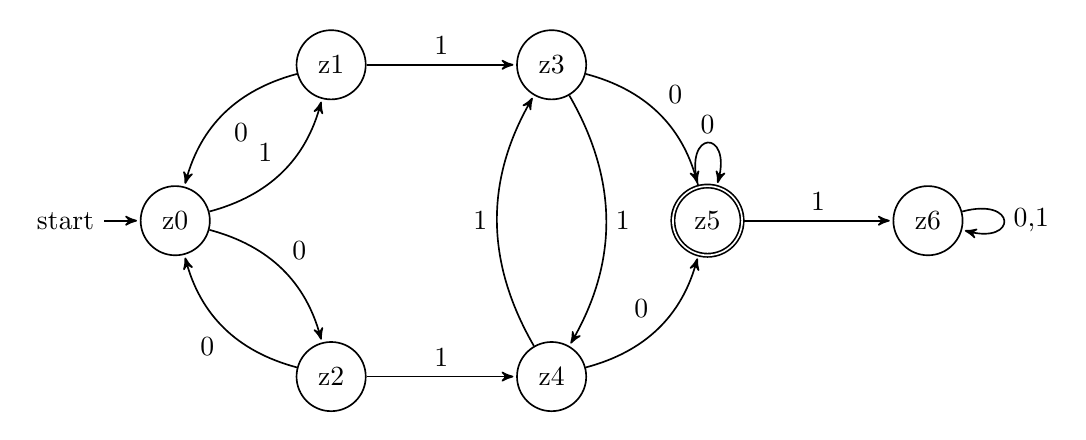
\begin{tikzpicture}[->,>=stealth',shorten >=1pt,auto,node distance=2.8cm,semithick]
        %   \tikzstyle{every state}=[fill=gray,draw=none,text=white]

        \node[initial,state]    (z0)               {z0};
        \node[state]            (z1) [above right of=z0] {z1};
        \node[state]            (z2) [below right of=z0] {z2};
        \node[state]            (z3) [right of=z1] {z3};
        \node[state]            (z4) [right of=z2] {z4};
        \node[state, accepting] (z5) [below right of=z3] {z5};
        \node[state]            (z6) [right of=z5] {z6};

        \path (z0) edge [bend left] node {0} (z2)
        edge [bend right] node {1} (z1)
        (z1) edge [bend right] node {0} (z0)
        edge node {1} (z3)
        (z2) edge [bend left] node {0} (z0)
        edge node {1} (z4)
        (z3) edge [bend left] node {0} (z5)
        edge [bend left] node {1} (z4)
        (z4) edge [bend right] node {0} (z5)
        edge [bend left] node {1} (z3)
        (z5) edge [loop above] node {0} (z5)
        edge node {1} (z6)
        (z6) edge [loop right] node {0,1} (z6);
    \end{tikzpicture}

    \section{Aufgabe 1}
    \subsection{a)}
    \begin{align*}
        L(A, z_0) &= \{11^*0^*,01^*0^* \mid \omega \in \Sigma^*\} \\
        L(A, z_1) &= \{1^*0^* \mid \omega \in \Sigma^*\} \\
        L(A, z_2) &= \{1^*0^* \mid \omega \in \Sigma^*\} \\
        L(A, z_3) &= \{1^*0^* \mid \omega \in \Sigma^*\} \\
        L(A, z_4) &= \{1^*0^* \mid \omega \in \Sigma^*\} \\
        L(A, z_5) &= \{0^* \mid \omega \in \Sigma^*\} \\
        L(A, z_6) &= \emptyset \\
    \end{align*}


    \subsection{b)}

    \begin{tabular}{c|ccccccc}
        ~ & $z_0$ & $z_1$ & $z_2$ & $z_3$ & $z_4$ & $z_5$ & $z_6$ \\
        \hline
        $z_0$ & \equiv    & X & X & X & X & X & X     \\
        $z_1$ & ~ & \equiv    & \equiv & X & X & X & X     \\
        $z_2$ & ~ & ~ & \equiv    & X & X & X & X     \\
        $z_3$ & ~ & ~ & ~ & \equiv    & \equiv & X & X     \\
        $z_4$ & ~ & ~ & ~ & ~ & \equiv    & X & X     \\
        $z_5$ & ~ & ~ & ~ & ~ & ~ & \equiv    & X     \\
        $z_6$ & ~ & ~ & ~ & ~ & ~ & ~ & \equiv    \\
    \end{tabular}
    \vspace{1cm}
    \begin{equation*}
        z_1 \equiv z_2 \;\text{und}\; z_3 \equiv z_4
    \end{equation*}

    \vspace{2cm}


    \subsection{c) Minimierter Automat}

    $\overline{A} = $

    \begin{tikzpicture}[->,>=stealth',shorten >=1pt,auto,node distance=2.8cm,
    semithick]
        %\tikzstyle{every state}=[fill=red,draw=none,text=white]

        \node[initial,state] (z0)                           {$z_0$};
        \node[state]         (z12) [right of=z0] {$z_{12}$};
        \node[state]                (z34) [right of=z12]     {$z_{34}$};
        \node[state,accepting]         (z5) [right of=z34]     {$z_5$};
        \node[state]         (z6) [right of=z5]       {$z_6$};


        \path
        (z0) edge [bend left]   node {0,1} (z12)
        (z12) edge [bend left]       node {0} (z0)
        edge node {1} (z34)
        (z34) edge node {0} (z5)
        edge [loop below]        node {1} (z3)
        (z5) edge node {1} (z6)
        edge [loop below]             node {0} (z5)
        (z6) edge [loop below]      node {0,1} (z2)
    \end{tikzpicture}

    \vspace{1cm}
    \subsection{d)}

    $\overline{A'} = $

    \begin{tikzpicture}[->,>=stealth',shorten >=1pt,auto,node distance=2.8cm,
    semithick]
        %\tikzstyle{every state}=[fill=red,draw=none,text=white]

        \node[initial,state] (z0)                           {$q_0$};
        \node[state]         (z12) [right of=z0] {$q_1$};
        \node[state]                (z34) [right of=z12]     {$q_2$};
        \node[state,accepting]         (z5) [right of=z34]     {$q_3$};
        \node[state]         (z6) [right of=z5]       {$q_4$};


        \path
        (z0) edge [bend left]   node {0,1} (z12)
        (z12) edge [bend left]       node {0} (z0)
        edge node {1} (z34)
        (z34) edge node {0} (z5)
        edge [loop below]        node {1} (z3)
        (z5) edge node {1} (z6)
        edge [loop below]             node {0} (z5)
        (z6) edge [loop below]      node {0,1} (z2)
    \end{tikzpicture}


    \newpage
    \section{Aufgabe 2}

    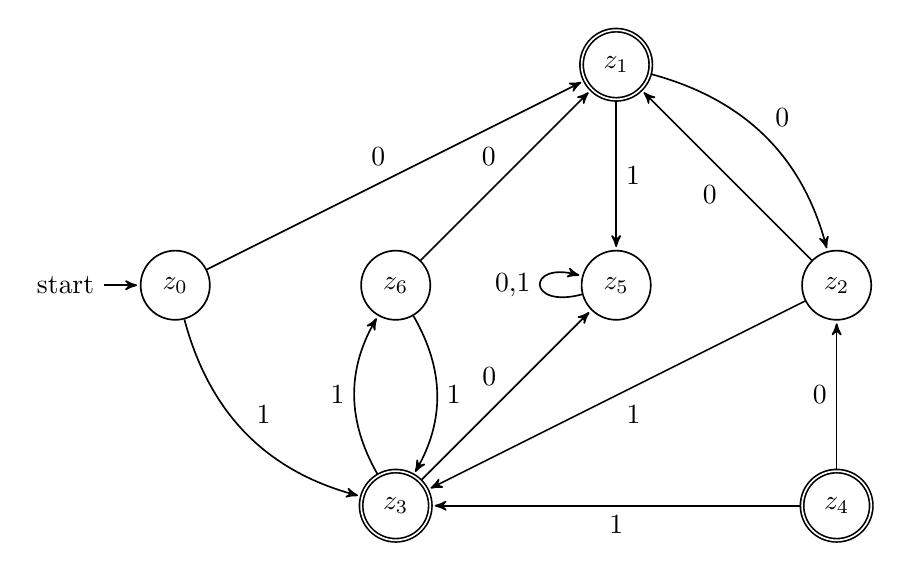
\begin{tikzpicture}[->,>=stealth',shorten >=1pt,auto,node distance=2.8cm,
    semithick]
        %\tikzstyle{every state}=[fill=red,draw=none,text=white]

        \node[initial,state] (z0)                           {$z_0$};
        \node[state]                (z6) [right of=z0]       {$z_6$};
        \node[state]                (z5) [right of=z6]       {$z_5$};
        \node[state,accepting]         (z3) [below of=z6]     {$z_3$};
        \node[state]                (z2) [right of=z5]     {$z_2$};
        \node[state,accepting]         (z1) [above of=z5] {$z_1$};
        \node[state,accepting]         (z4) [below of=z2]       {$z_4$};

        \path (z0) edge node {0} (z1)
        edge [bend right] node {1} (z3)
        (z1) edge [bend left] node {0} (z2)
        edge node {1} (z5)
        (z2) edge node {0} (z1)
        edge node {1} (z3)
        (z3) edge node {0} (z5)
        edge [bend left] node {1} (z6)
        (z4) edge node {0} (z2)
        edge node {1} (z3)
        (z5) edge [loop left]       node {0,1} (z5)
        (z6) edge node {0} (z1)
        edge [bend left] node {1} (z3);
    \end{tikzpicture}

    \subsection{Entfernung von unerreichbaren Nodes}


    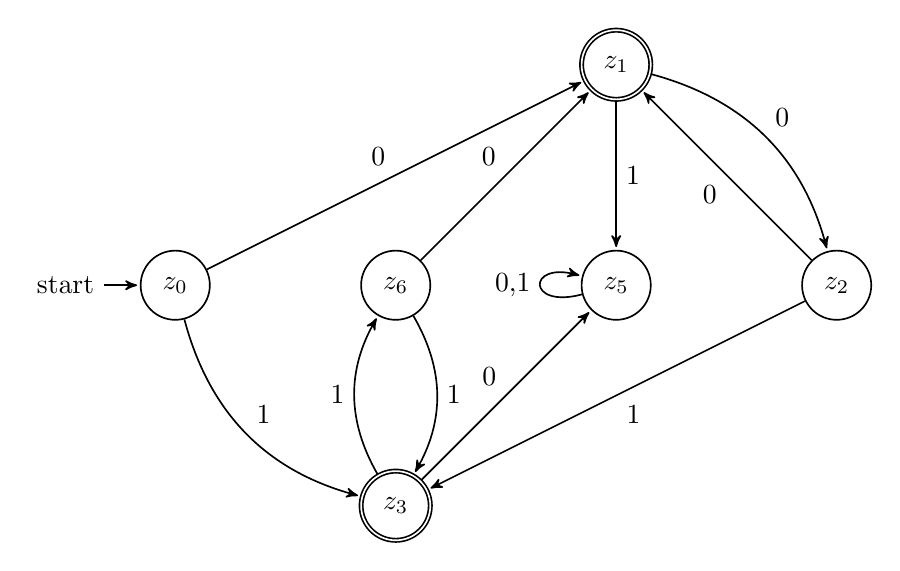
\begin{tikzpicture}[->,>=stealth',shorten >=1pt,auto,node distance=2.8cm,
    semithick]
        %\tikzstyle{every state}=[fill=red,draw=none,text=white]

        \node[initial,state] (z0)                           {$z_0$};
        \node[state]                (z6) [right of=z0]       {$z_6$};
        \node[state]                (z5) [right of=z6]       {$z_5$};
        \node[state,accepting]         (z3) [below of=z6]     {$z_3$};
        \node[state]                (z2) [right of=z5]     {$z_2$};
        \node[state,accepting]         (z1) [above of=z5] {$z_1$};

        \path (z0) edge node {0} (z1)
        edge [bend right] node {1} (z3)
        (z1) edge [bend left] node {0} (z2)
        edge node {1} (z5)
        (z2) edge node {0} (z1)
        edge node {1} (z3)
        (z3) edge node {0} (z5)
        edge [bend left] node {1} (z6)
        (z5) edge [loop left]       node {0,1} (z5)
        (z6) edge node {0} (z1)
        edge [bend left] node {1} (z3);
    \end{tikzpicture}

    \newpage
    \begin{tabular}{c|cccccc}
        ~ & $z_0$ & $z_1$ & $z_2$ & $z_3$ & $z_5$ & $z_6$ \\
        \hline
        $z_0$ & \equiv& X & \equiv & X & X & X     \\
        $z_1$ & ~ & \equiv& X & X & X & X     \\
        $z_2$ & ~ & ~ & \equiv& X & X & \equiv     \\
        $z_3$ & ~ & ~ & ~ & \equiv& X & X     \\
        $z_5$ & ~ & ~ & ~ & ~ & \equiv& X     \\
        $z_6$ & ~ & ~ & ~ & ~ & ~ & \equiv    \\
    \end{tabular}
    \vspace{1cm}
    \begin{equation*}
        z_2 \equiv z_0 \;\text{und}\; z_2 \equiv z_6
    \end{equation*}

    \vspace{2cm}

    \subsection{Minimierter Automat}

    \begin{tikzpicture}[->,>=stealth',shorten >=1pt,auto,node distance=2.8cm, semithick]
        %\tikzstyle{every state}=[fill=red,draw=none,text=white]

        \node[initial,state]        (z2)                   {$z_{026}$};
        \node[state,accepting]      (z1) [above of=z2]     {$z_1$};
        \node[state,accepting]      (z3) [below of=z2]     {$z_3$};
        \node[state]                (z5) [right of=z2]     {$z_5$};

        \path (z1) edge [bend left] node {0} (z2)
        edge node {1} (z5)
        (z2) edge node {0} (z1)
        edge node {1} (z3)
        (z3) edge node {0} (z5)
        edge [bend left] node {1} (z2)
        (z5) edge [loop right]       node {0,1} (z5)
    \end{tikzpicture}


\end{document}
